\documentclass[10pt,twoside]{article}

\usepackage[letterpaper,margin=0.76in,headheight=20pt]{geometry}
\usepackage{newtxtext,newtxmath}
\usepackage{microtype}
\usepackage{xcolor}
\usepackage{graphicx}
\usepackage{booktabs}
\usepackage{tabularx}
\usepackage{array}
\usepackage{tikz}
\usetikzlibrary{arrows.meta,positioning,fit,backgrounds}
\usepackage{pgfplots}
\pgfplotsset{compat=1.18}
\usepackage{hyperref}
\usepackage{xurl}
\usepackage{fancyhdr}
\usepackage{titlesec}
\usepackage{enumitem}
\usepackage{caption}
\usepackage{float}

\definecolor{vlteal}{HTML}{16615A}
\definecolor{vltealdark}{HTML}{0E4742}
\definecolor{vllight}{HTML}{E9F5F0}
\definecolor{vlpaper}{HTML}{FBFAF7}
\definecolor{vltext}{HTML}{16181D}
\definecolor{vlmuted}{HTML}{626A76}
\definecolor{vlrule}{HTML}{D8D4CB}
\definecolor{vlgold}{HTML}{A57A18}
\definecolor{vlred}{HTML}{B14949}

\hypersetup{
  colorlinks=true,
  linkcolor=vltealdark,
  citecolor=vltealdark,
  urlcolor=vlteal,
  pdftitle={Voice-Light: From Conversational Data to a Deployed Streaming Voice Agent},
  pdfauthor={Bertil Braun}
}

\pagestyle{fancy}
\fancyhf{}
\fancyhead[LE,LO]{\small\color{vlmuted}VOICE-LIGHT TECHNICAL REPORT}
\fancyhead[RE,RO]{\small\color{vlmuted}SEPTEMBER 2026}
\fancyfoot[C]{\small\color{vlmuted}\thepage}
\renewcommand{\headrulewidth}{0.3pt}
\renewcommand{\headrule}{\hbox to\headwidth{\color{vlrule}\leaders\hrule height \headrulewidth\hfill}}
\fancypagestyle{plain}{%
  \fancyhf{}
  \fancyhead[LE,LO]{\small\color{vlmuted}VOICE-LIGHT TECHNICAL REPORT}
  \fancyhead[RE,RO]{\small\color{vlmuted}SEPTEMBER 2026}
  \fancyfoot[C]{\small\color{vlmuted}\thepage}
  \renewcommand{\headrulewidth}{0.3pt}}

\titleformat{\section}{\Large\bfseries\color{vltealdark}}{\thesection}{0.6em}{}
\titleformat{\subsection}{\large\bfseries\color{vltext}}{\thesubsection}{0.55em}{}
\titlespacing*{\section}{0pt}{1.4em}{0.55em}
\titlespacing*{\subsection}{0pt}{1.1em}{0.35em}

\setlength{\parindent}{0pt}
\setlength{\parskip}{0.48em}
\setlist[itemize]{leftmargin=1.3em,itemsep=0.18em,topsep=0.3em}
\setlist[enumerate]{leftmargin=1.45em,itemsep=0.25em,topsep=0.3em}
\DeclareCaptionFont{vlmuted}{\color{vlmuted}}
\DeclareCaptionFont{vltealdark}{\color{vltealdark}}
\captionsetup{font={small,vlmuted},labelfont={bf,vltealdark}}

\newcommand{\VoiceLight}{\textsc{Voice-Light}}
\newcommand{\code}[1]{\texttt{#1}}
\newcommand{\keyresult}[2]{%
  \begin{minipage}[t]{0.235\textwidth}
    \centering
    {\Large\bfseries\color{vlteal}#1}\par
    \vspace{0.15em}
    {\small\color{vlmuted}#2}
  \end{minipage}}

\begin{document}

\begin{titlepage}
  \pagecolor{vlpaper}
  \vspace*{0.6in}
  {\color{vlteal}\rule{\textwidth}{5pt}}\\[0.55in]
  {\fontsize{18}{20}\selectfont\bfseries\color{vlteal}VOICE-LIGHT}\\[0.22in]
  {\fontsize{34}{39}\selectfont\bfseries\color{vltext}
    From conversational data to a\\deployed streaming voice agent\par}
  \vspace{0.35in}
  {\Large\color{vlmuted}
    Synthetic generation, automatic annotation, causal turn-taking,
    latency engineering, and scale-to-zero deployment\par}
  \vfill
  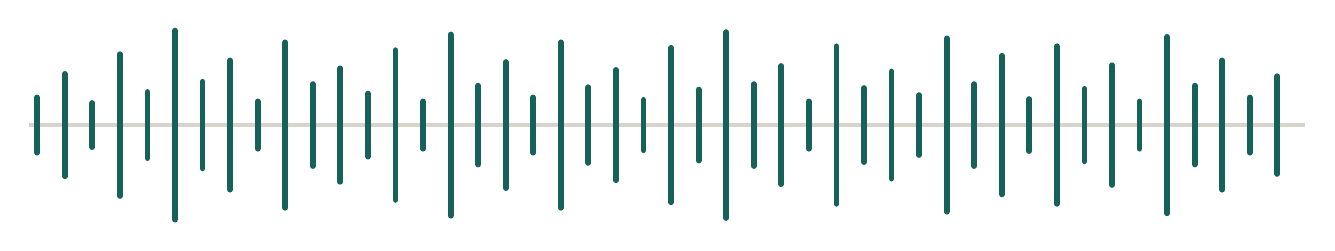
\begin{tikzpicture}[x=1cm,y=1cm]
    \draw[vlrule,line width=1.2pt] (0,0) -- (16.2,0);
    \foreach \x/\h in {0.1/0.35,0.45/0.65,0.8/0.28,1.15/0.9,1.5/0.42,1.85/1.2,2.2/0.55,2.55/0.82,2.9/0.3,3.25/1.05,3.6/0.52,3.95/0.72,4.3/0.4,4.65/0.95,5/0.3,5.35/1.15,5.7/0.5,6.05/0.8,6.4/0.35,6.75/1.05,7.1/0.48,7.45/0.7,7.8/0.32,8.15/0.98,8.5/0.45,8.85/1.18,9.2/0.52,9.55/0.75,9.9/0.3,10.25/1.0,10.6/0.47,10.95/0.68,11.3/0.38,11.65/1.1,12/0.52,12.35/0.88,12.7/0.33,13.05/1.0,13.4/0.46,13.75/0.76,14.1/0.3,14.45/1.12,14.8/0.5,15.15/0.82,15.5/0.35,15.85/0.62}
      \draw[vlteal,line width=2.1pt,line cap=round] (\x,-\h) -- (\x,\h);
  \end{tikzpicture}
  \vfill
  {\large\bfseries Bertil Braun}\par
  {\color{vlmuted}Technical report, version 1.0 \textbullet\ September 2026}\par
  \vspace{0.25in}
  \href{https://voice.bertil-braun.de}{voice.bertil-braun.de}\quad
  \href{https://github.com/BertilBraun/Voice-Light}{github.com/BertilBraun/Voice-Light}
  \vspace{0.4in}
\end{titlepage}
\nopagecolor

\begin{abstract}
\VoiceLight{} is an end-to-end investigation of natural, low-latency interaction in a cascaded
voice agent. The project covers structured synthetic conversation generation, automatic
enrichment of human conversational audio, fine-tuning a language model for spoken tool use,
training a causal adapter over a streaming speech encoder, locked offline evaluation, full-duplex
playback control, and a public two-GPU Modal deployment. The strongest result is the complete,
measured development loop rather than a claim that every learned component surpassed its
baseline. A Qwen3-1.7B LoRA substantially improved tool protocol behavior on its synthetic
holdout, yet a stronger Qwen3-4B checkpoint was retained for production quality. The turn adapter
learned useful causal interaction evidence, yet its completion policy did not beat Silero or
LiveKit timing baselines on the locked real-conversation benchmark; production therefore uses a
hybrid controller. In a final eight-turn microphone session, every turn completed and six reached
browser PCM within 800 ms of speech end, with a 677 ms median. The report documents the positive
results, reversals, latency work, and limitations that produced the deployed system.
\end{abstract}

\begin{center}
  \keyresult{3,999}{typed synthetic tool-use conversations}\hfill
  \keyresult{183k}{approximately, turn-adapter parameters}\hfill
  \keyresult{677 ms}{median speech end to browser PCM}\hfill
  \keyresult{8/8}{completed final microphone turns}
\end{center}

\vspace{0.5em}
\tableofcontents

\section{Problem and design goals}

A conventional voice assistant is often drawn as a serial pipeline: automatic speech recognition
(ASR), then a language model, then text-to-speech (TTS). That abstraction hides the interaction
problem. A usable conversational system must decide whether a silence is a completed turn or a
within-turn hesitation; react immediately when speech begins during playback without canceling on
every short acknowledgment; ensure canceled audio cannot reappear; and distinguish generated text
from speech that actually reached the listener.

\VoiceLight{} began with an aspirational 250--600 ms speech-end-to-first-audio budget. The budget
was deliberately decomposed into endpoint confirmation, language-model response formation, speech
synthesis, transport, and browser playback. These stages overlap in the final system, so their
individual medians must not be added. The project instead uses monotonic timestamps and audio
sample positions to expose both critical-path latency and private work completed before a turn is
committed.

The design goals were:

\begin{itemize}
  \item stream audio, ASR, text generation, synthesis, and playback rather than batch each stage;
  \item preserve strict causality in training, evaluation, and runtime inference;
  \item support ordinary turns, hesitation, short backchannels, and deliberate interruption;
  \item make early reactions reversible until enough evidence exists to cancel the assistant;
  \item run structured and sequential tools without speaking protocol markup;
  \item retain only assistant speech acknowledged by the browser in durable history;
  \item degrade to ASR and conservative timing if the learned adapter fails; and
  \item scale to zero for an intermittently visited public demonstration.
\end{itemize}

The work follows the broader observation that turn-taking depends on future interaction structure,
not only present speech activity. Voice Activity Projection models future speaker activity
\cite{vap}, while acoustic and language-model fusion has shown that prosodic and lexical evidence
can be complementary \cite{acousticllm}. \VoiceLight{} explores a narrower engineering question:
how much of that interaction evidence can be attached to an existing streaming ASR backbone and
then used safely inside a real playback controller?

\section{One project, two data pipelines}

\begin{figure}[H]
\centering
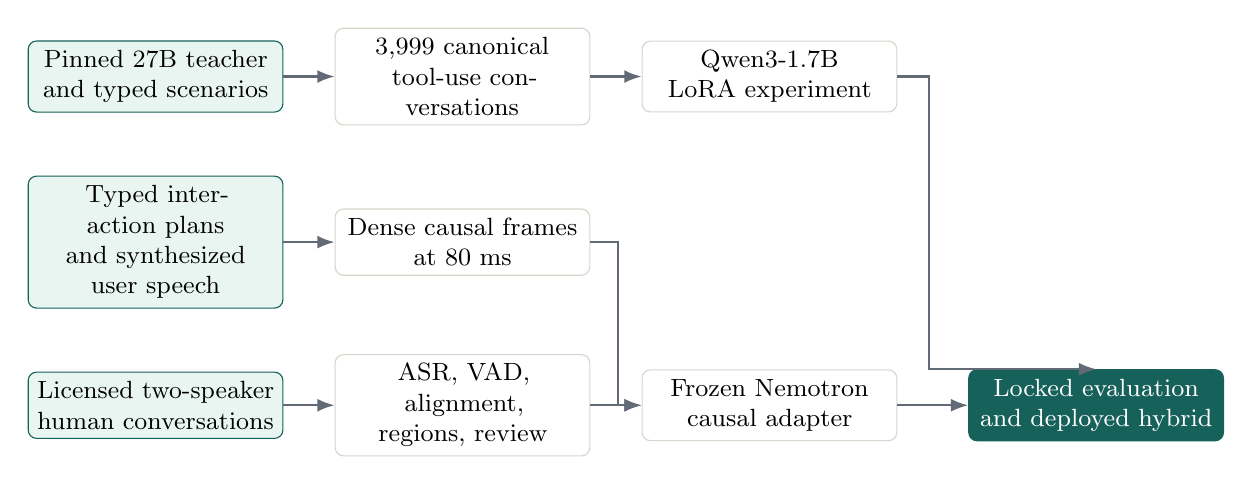
\begin{tikzpicture}[
  node distance=0.55cm and 0.65cm,
  box/.style={draw=vlrule,rounded corners=3pt,fill=white,minimum height=0.75cm,text width=3.0cm,align=center,font=\small},
  source/.style={box,fill=vllight,draw=vlteal},
  arrow/.style={-{Latex[length=2.2mm]},line width=0.8pt,color=vlmuted}
]
  \node[source] (toolsource) {Pinned 27B teacher\\and typed scenarios};
  \node[box,right=of toolsource] (tooldata) {3,999 canonical\\tool-use conversations};
  \node[box,right=of tooldata] (lora) {Qwen3-1.7B\\LoRA experiment};
  \node[source,below=0.8cm of toolsource] (audiosource) {Typed interaction plans\\and synthesized user speech};
  \node[box,right=of audiosource] (synthdata) {Dense causal frames\\at 80 ms};
  \node[source,below=0.8cm of audiosource] (human) {Licensed two-speaker\\human conversations};
  \node[box,right=of human] (annotation) {ASR, VAD, alignment,\\regions, review};
  \node[box,right=of annotation] (turn) {Frozen Nemotron\\causal adapter};
  \node[box,fill=vlteal,text=white,draw=vlteal,right=0.9cm of turn] (deploy) {Locked evaluation\\and deployed hybrid};
  \draw[arrow] (toolsource) -- (tooldata);
  \draw[arrow] (tooldata) -- (lora);
  \draw[arrow] (audiosource) -- (synthdata);
  \draw[arrow] (human) -- (annotation);
  \draw[arrow] (synthdata.east) -- ++(0.35,0) |- (turn.west);
  \draw[arrow] (annotation) -- (turn);
  \draw[arrow] (turn) -- (deploy);
  \draw[arrow] (lora.east) -- ++(0.4,0) |- (deploy.north);
\end{tikzpicture}
\caption{The report follows two training branches into one evaluated deployment. Synthetic and
human evidence remain distinguishable throughout the pipeline.}
\label{fig:pipeline}
\end{figure}

\subsection{Synthetic spoken tool use}

Spoken tool use was treated as a data and protocol problem rather than a prompt-only feature. A
pinned \code{Qwen3.6-27B-FP8} teacher generated provider-neutral records for natural
conversation, drafting, brainstorming, search, calculation, time queries, sequential calls, and
correction or recovery. The production run planned 4,000 scenarios and accepted 3,999; one request
ended in an HTTP read timeout. The resulting corpus contains 11,810 user messages, 15,308 assistant
messages, and 3,498 structured calls across \code{search}, \code{calculate}, and \code{get\_time}.

Generation used a causal conversation state machine. The teacher produced a user turn and then
either assistant speech or speech followed by a typed call. The controller executed or synthesized
the result, appended the linked call and result, and only then requested the next assistant step.
Calculator and time results were deterministic. Synthetic search results came from the teacher,
not the live web; consequently, the corpus teaches call ordering and grounding to supplied text,
not factual retrieval quality.

The canonical JSONL is semantic rather than tokenized. It stores runtime tool definitions, audible
assistant text, typed calls, stable identifiers, outcomes, later turns, split metadata, provenance,
and hashes. The run pins the teacher revision, prompt revision, source commit, scenario seeds,
quantization, and time anchor. Structural checks retained schema validity, causal call/result order,
deterministic tool checks, spoken-length limits, and protocol-leak detection. Subjective
teacher-based rejection was disabled after manual review found its false positives
counterproductive.

\subsection{Synthetic conversational turn-taking audio}

The second generator models coherent conversation timelines rather than isolated completion
utterances. Typed plans distinguish five semantic conditions: genuine user completion, a HOLD
pause followed by continuation, non-floor feedback during assistant speech, a response after the
assistant yields, and deliberate interruption. The plan also contains ordinary event-free user,
assistant, and silence spans.

Only user audio is synthesized. Virtual assistant text keeps the scenario coherent and estimates
assistant duration, but assistant waveform never becomes an input artifact. The runtime-relevant
assistant-speaking probability is compiled as a causal state curve with ramps, dips, and bounded
noise. This prevents future assistant state or clean synthetic timing from leaking into the
adapter.

The accepted rendering route used Qwen VoiceDesign references to condition CosyVoice 3 zero-shot
voices. Qwen Base ICL cloning was rejected for robotic speech, while IndexTTS 2.5, Chatterbox, and
VoXtream were rejected in listening gates. Each user unit was rendered and trimmed independently;
the compiler then measured its active speech, assembled the final timeline, and rasterized
20-second views into 250 frames at 80 ms. A planned pause became HOLD supervision only if the
rendered unit contained at least 500 ms of silence followed by resumed speech.

The public synthetic repository stores lossless speech units and reconstruction metadata rather
than duplicating every composed waveform. Plans, voice provenance, trim measurements, composition
seeds, split assignments, and checksums allow conversation audio and training crops to be rebuilt.
The retained V4 and V5 manifests contain 1,092 and 1,097 timelines, approximately 21.84 and 21.80
hours of source timeline respectively. These counts describe retained run manifests, not a claim
that synthetic interaction validation substitutes for natural conversation.

\subsection{Automatic preparation of human conversations}

The human pipeline separates three artifact layers: authorized source audio, recording-level
evidence, and materialized training windows. Each complete speaker track is stored once as lossless
FLAC. Typed Parquet rows reference bounded 20-second intervals and contain aligned inputs, targets,
and masks; they do not duplicate the recording.

Ingestion registers and hashes both channels, reuses exact cached transcripts, transports only
missing material, applies a reviewed inter-speaker offset, and persists a full-duration annotation
and quality result transactionally. Independent ASR and activity evidence includes Parakeet,
Canary, faster-Whisper, Nemotron, VAD, multi-model consensus, channel-aware crosstalk filtering,
conversation regions, and quality flags. Supplied Mundo TurnBench human annotations remain an
independent evidence source rather than being copied into model-output fields to manufacture
agreement.

The prepared sources included eight accepted MagicHub conversations (about 2.77 hours) and 37
accepted Mundo TurnBench conversations (about 7.31 hours); a silent TurnBench recording was
excluded. Splits are conversation-disjoint. The first manual plumbing gate reviewed 12
dataset-stratified recordings and retained its final items after specific exclusions. It was not a
comprehensive audit of every split, category, or rejection reason, and the report does not present
it as one.

\section{Models and training}

\subsection{A language adapter for spoken tools}

The tool-use experiment fine-tuned \code{Qwen/Qwen3-1.7B} with a BF16 rank-16 LoRA. Two source
records from each combination of eight behavior families and five speech styles formed a balanced
80-record validation split; the remaining 3,919 records were training data. Across 16 deterministic
passes, every record appeared once per pass. Intact short segments were regrouped into histories
with 8--16 user turns, producing 14,391 training histories and 17.84 million rendered tokens, of
which 6.86 million were assistant targets.

The native Qwen chat template rendered the canonical records with thinking disabled. The loss mask
retained ordinary assistant speech, the spoken bridge preceding a call, structured call tokens,
post-result continuation, and later assistant turns. System text, tool definitions, user messages,
tool results, padding, and non-assistant protocol tokens were masked. The adapter targeted all
attention and MLP projections, trained 17.43 million parameters, and completed 904 optimizer steps
in 47 minutes on an RTX 4090.

Validation loss reached its minimum after approximately four logical passes and then increased,
while free-generation task metrics continued to improve. This mismatch made validation loss an
unsafe sole checkpoint selector. It also exposed the narrower limitation: learning the synthetic
protocol did not imply improved general reasoning. A later production canary favored the stronger
Qwen3-4B Instruct checkpoint, which is what the public deployment uses. The LoRA remains a
published, reproducible training result rather than the deployed conversation model.

\subsection{A causal adapter on shared Nemotron features}

The turn-taking model attaches approximately 183,000 trainable parameters to the frozen
\code{Nemotron Speech Streaming 0.6B} encoder. Nemotron is a cache-aware streaming
FastConformer-RNNT. Its activation caches allow new non-overlapping chunks to reuse prior work
\cite{stateful,fastconformer}. This property made it possible to share one streaming backbone
between ASR and turn inference rather than re-encoding a rolling waveform or loading a second
0.6-billion-parameter model.

The adapter taps encoder layers 6, 12, 18, and 24. Each 1,024-dimensional tap is normalized and
projected to 32 dimensions; the streams are fused to 64 dimensions, processed by residual causal
depthwise-separable convolutions, combined with assistant-speaking state, and passed through a
single-layer 64-dimensional unidirectional GRU. Separate heads emit completion/yield evidence,
interaction events including floor take and non-floor feedback, and future activity. Convolution
and recurrent state persist incrementally and reset with the ASR stream.

Synthetic pretraining selected step 2,250. Completion AUROC was 0.9260 on held-out synthetic
conversation but only 0.5646 on human validation, demonstrating a large domain gap. Human
fine-tuning warm-started those weights with a fresh optimizer, 15\% synthetic replay, and 1,884
human boundaries: 1,038 HOLD and 846 EOT. The 750-step run improved human AUROC to 0.5972 and
risk-constrained EOT recall from 47.48\% to 65.04\%, while false cutoffs moved from 4.48\% to
3.73\%. Human p95 commitment latency remained 2.0 seconds.

The final \code{adapter-best.pt} is step 750, pinned to Nemotron revision
\code{ebe59e5a817142986528bbbee5dba8db7b38ed50}, one lookahead token, 80 ms encoder frames, and the
four taps above. Human validation selected it; synthetic validation could not. At runtime, forward
hooks capture the exact features produced by persistent streaming ASR. A bounded latest-value queue
supersedes stale adapter work, and loading or inference failure degrades the predictor without
stopping ASR or the voice session.

\section{Evaluation changed the product}

The project uses separate evaluation contracts for separate claims. Tool-use generation measures
behavior on held-out synthetic conversation states. The historical V1 turn benchmark evaluates
future silence through the original yield target and locks a validation-selected policy before
opening test. V2 evaluates semantic completion at speech boundaries; it stopped at validation after
no detector met the predefined deployment gate. Deployment acceptance is a human microphone smoke
test, not a substitute for a controlled conversational study.

\subsection{Tool-use proof of concept}

\begin{table}[H]
\centering
\caption{Original balanced synthetic holdout for the Qwen3-1.7B LoRA.}
\begin{tabularx}{0.82\textwidth}{Xrr}
\toprule
Behavior & Base & Final adapter \\
\midrule
Correct tool decision & 80.0\% & \textbf{95.2\%} \\
Exact tool name & 78.6\% & \textbf{94.3\%} \\
Valid argument schema & 80.0\% & \textbf{95.2\%} \\
Concise 1--12-word bridge & 7.6\% & \textbf{94.3\%} \\
Correctly avoided a tool & 70.0\% & \textbf{100.0\%} \\
Valid post-tool continuation & 98.3\% & \textbf{100.0\%} \\
\bottomrule
\end{tabularx}
\label{tab:tool}
\end{table}

Across three decoding seeds, the final adapter emitted 200 of 210 expected calls, selected the
exact tool for 198, produced 200 schema-valid required calls, avoided a tool in all 90 no-tool
states, and continued after all 180 tool results. The result demonstrates acquisition of the
generator's conversational protocol. It does not establish factual accuracy, robust web search, or
general tool intelligence because evaluation points share the synthetic generator and schema.

\begin{figure}[H]
\centering
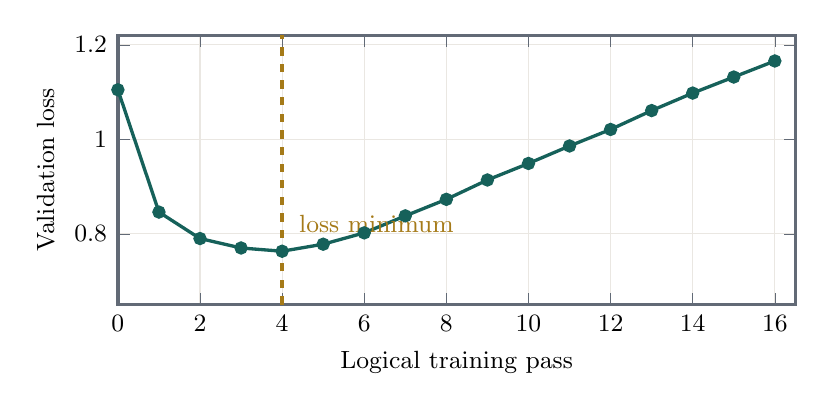
\begin{tikzpicture}
\begin{axis}[
  width=0.84\textwidth,height=5.0cm,
  xlabel={Logical training pass},ylabel={Validation loss},
  xmin=0,xmax=16.5,ymin=0.65,ymax=1.22,
  grid=major,grid style={vlrule!55},
  axis line style={vlmuted},tick style={vlmuted},
  label style={font=\small},tick label style={font=\small},
  line width=1.2pt
]
\addplot[color=vlteal,mark=*,mark size=1.8pt] coordinates {
 (0,1.105) (1,0.846) (2,0.790) (3,0.770) (4,0.7631) (5,0.778)
 (6,0.802) (7,0.838) (8,0.873) (9,0.914) (10,0.949) (11,0.986)
 (12,1.021) (13,1.061) (14,1.098) (15,1.132) (16,1.1660)};
\addplot[color=vlgold,dashed] coordinates {(4,0.65) (4,1.22)};
\node[anchor=south west,font=\small,color=vlgold] at (axis cs:4.15,0.78) {loss minimum};
\end{axis}
\end{tikzpicture}
\caption{Teacher-forced validation loss bottomed early, then rose. Behavioral checkpoint
selection remained necessary; improving task behavior does not make the overfitting irrelevant.}
\label{fig:loss}
\end{figure}

\subsection{Locked turn-detection benchmark}

The locked V1 test contains 1,673 causal silence candidates from 11 conversations, including only
37 HOLD cases. Threshold, minimum delay, and timeout were selected on validation and frozen before
test. Table~\ref{tab:v1} shows the central negative result: the Voice-Light checkpoint preserved a
low false-cutoff rate but crossed its learned threshold on only 205 of 1,636 EOT cases. Most turns
therefore used the 800 ms timeout, and the learned policy did not beat the Silero or LiveKit timing
baselines.

\begin{table}[H]
\centering
\caption{Historical locked V1 real-conversation test. Smart Turn has known source-overlap risk and
is shown only as contextual evidence.}
\small
\begin{tabularx}{\textwidth}{Xrrrr}
\toprule
Detector & False cutoff & EOT recall & Mean latency & Policy \\
\midrule
Voice Light step 3,500 & 2.70\% (1/37) & 12.53\% & 770 ms & 0.90 / 560 / 800 \\
Silero VAD 6.2.1 & 2.70\% (1/37) & \textbf{95.60\%} & 656 ms & 0.05 / 640 / 800 \\
Smart Turn 3.2 & 13.51\% (5/37) & 20.72\% & 684 ms & 0.95 / 80 / 800 \\
LiveKit v1-mini & 2.70\% (1/37) & 91.50\% & \textbf{654 ms} & 0.15 / 640 / 800 \\
\bottomrule
\end{tabularx}
\label{tab:v1}
\end{table}

The V2 semantic-completion validation set retained 134 HOLD and 655 EOT examples after ignoring
216 ambiguous cases. Voice-Light step 3,500 achieved 3.73\% false cutoffs, 65.80\% EOT recall,
1,732 ms mean latency, 0.6866 AUROC, and 0.8993 AP. EOT prevalence was already 83.02\%, so AP was
only modestly above a constant prevalence reference. No detector met the joint gate of at most 5\%
false cutoff, at least 70\% recall, and at most 800 ms p95 latency; V2 test therefore remained
unopened.

A completion-primary retrain improved AP, calibration, and recall but still missed the gate. Step
625 reached 0.6864 AUROC, 0.9052 AP, 4.48\% false cutoffs, and 69.01\% EOT recall, with a 2.0-second
p95. Training to step 3,000 reduced recall. This rejected both "use the old target longer" and
"train the new target longer" as sufficient production strategies.

\subsection{Threats to validity}

Several constraints limit interpretation:

\begin{itemize}
  \item The tool-use holdout shares the synthetic generator, ontology, and protocol with training.
  Its three seeds repeat generation over a smaller set of states rather than creating independent
  tasks.
  \item Synthetic search answers came from the teacher. They do not measure live retrieval,
  citation quality, adversarial results, or provider latency.
  \item Turn candidates from only 11 conversations are correlated. On the locked test, one HOLD
  error changes the false-cutoff rate by 2.70 percentage points.
  \item Smart Turn and Voice-Light both include Mundo-derived material; the baseline cannot support
  a clean superiority comparison without exact source-audio auditing.
  \item The V2 completion inventory uses heuristic confidence bands and leaves 216 ambiguous cases
  out of scoring. The planned independent human label audit remains incomplete.
  \item The final microphone result is one acceptance session. It has no separately timestamped
  final-topology duck, cancellation, or backchannel-resume events.
\end{itemize}

These limitations are part of the result. They directly constrain the claims made here and explain
why the deployed system is hybrid.

\section{Deployed streaming system}

\begin{figure}[H]
\centering
\resizebox{\textwidth}{!}{%
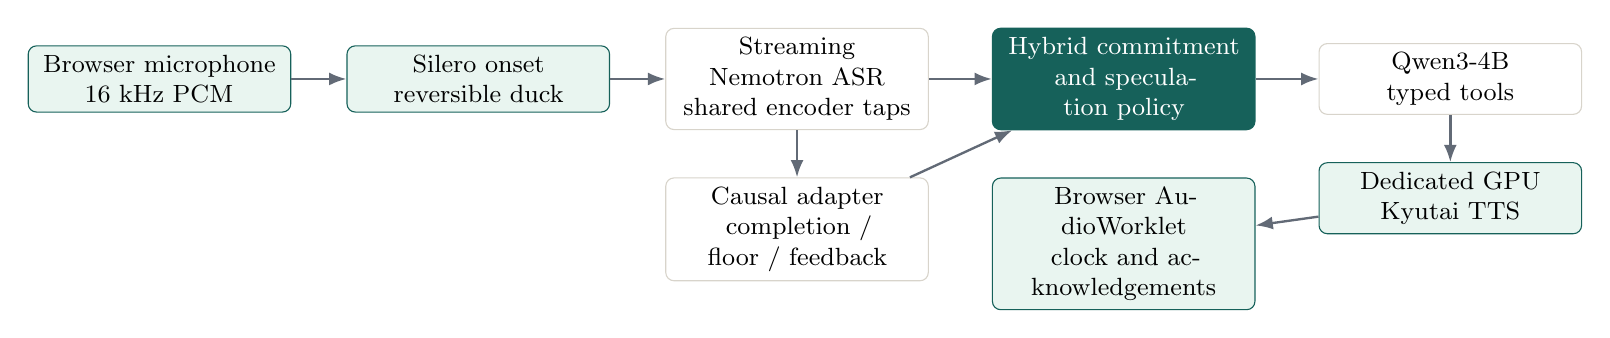
\begin{tikzpicture}[
  node distance=0.45cm and 0.7cm,
  box/.style={draw=vlrule,rounded corners=3pt,fill=white,minimum height=0.75cm,text width=3.1cm,align=center,font=\small},
  green/.style={box,fill=vllight,draw=vlteal},
  dark/.style={box,fill=vlteal,draw=vlteal,text=white},
  arrow/.style={-{Latex[length=2.2mm]},line width=0.85pt,color=vlmuted}
]
  \node[green] (browser) {Browser microphone\\16 kHz PCM};
  \node[green,right=of browser] (silero) {Silero onset\\reversible duck};
  \node[box,right=of silero] (nemotron) {Streaming Nemotron ASR\\shared encoder taps};
  \node[box,below=0.6cm of nemotron] (adapter) {Causal adapter\\completion / floor / feedback};
  \node[dark,right=0.8cm of nemotron] (policy) {Hybrid commitment\\and speculation policy};
  \node[box,right=0.8cm of policy] (qwen) {Qwen3-4B\\typed tools};
  \node[green,below=0.6cm of qwen] (tts) {Dedicated GPU\\Kyutai TTS};
  \node[green,below=0.6cm of policy] (playback) {Browser AudioWorklet\\clock and acknowledgements};
  \draw[arrow] (browser) -- (silero);
  \draw[arrow] (silero) -- (nemotron);
  \draw[arrow] (nemotron) -- (policy);
  \draw[arrow] (nemotron) -- (adapter);
  \draw[arrow] (adapter) -- (policy);
  \draw[arrow] (policy) -- (qwen);
  \draw[arrow] (qwen) -- (tts);
  \draw[arrow] (tts) -- (playback);
\end{tikzpicture}
}
\caption{Production runtime. Immediate acoustic reaction and learned interaction evidence meet at
a typed controller; browser playback remains the authority on what was heard.}
\label{fig:runtime}
\end{figure}

\subsection{Hybrid overlap policy}

Silero remains the immediate acoustic authority. When user speech begins during assistant playback,
the browser fades toward -15 dB over 450 ms and pauses by 500 ms. This response is reversible: onset
alone does not discard generation. A floor-take probability above the configurable 0.82 threshold
can commit interruption and cancellation. A non-floor-feedback probability above 0.82 becomes
actionable after the short speech burst ends and resumes the same generation without adding a user
turn. Explicit stop, repair, question, or meaningful lexical evidence provides another fast path.

Ambiguous overlap is bounded. Sustained speech commits floor taking after 900 ms, while a short
ended burst resolves conservatively as non-floor feedback. Empty or slow final ASR receives a
120 ms grace rather than parking playback indefinitely. Generation and TTS budgets are held after
350 ms of unresolved overlap, and paused audio remains resumable for at most 800 ms. A committed
interruption rejects new server PCM immediately and fades no more than 100 ms of already-buffered
audio.

The adapter does not continuously encode assistant-only silence. It catches up from a bounded
pre-roll after Silero detects user activity, using the same persistent Nemotron stream once active.
This preserves one backbone and strict causality, but limits the acoustic context available at the
earliest overlap decision.

\subsection{Speculation and cancellation}

After 80 ms of low Silero speech probability, the adapter receives another 80 ms opportunity to
open a speculative response candidate. If learned evidence is not ready, a Silero fallback may
start at 160 ms. Candidate text and PCM remain private until final ASR and transcript-revision checks
permit promotion. Revisions limited to case, punctuation, whitespace, or apostrophes preserve work;
lexical change invalidates it.

Instrumentation showed why this helps inconsistently. In one session, 24 candidates were created
and six promoted. Qwen text was ready at commitment for 60\% of promoted candidates, but TTS PCM
was ready for none. Median candidate lead over the final Silero endpoint was only 11.6 ms, while
candidate-to-PCM time was 855 ms. Speculation often hid Qwen work but could not remove Kyutai's
fixed first-frame computation.

The system uses generation identifiers, cancellation barriers, and rebased sample positions to
reject stale text or PCM. Playback clocks and boundary acknowledgements return every 80 ms. Durable
assistant history is constructed only from audio ranges that the browser confirms it rendered;
generated but canceled words remain diagnostic evidence rather than conversation content.

\subsection{Tool execution and speech boundaries}

Structured tools support calculation, current time, and web search, including sequential rounds.
Tool execution can overlap with bridge audio already buffered in the browser. Kyutai, however,
requires text lookahead. The bridge must therefore be closed before awaiting a tool result, and the
result begins a second TTS utterance within the same assistant generation. Reusing one uninterrupted
TTS session was implemented and reverted because it could strand the last bridge words until tool
completion, producing a deterministic mid-preamble stall. The final design avoids that stall but
can retain a short acoustic seam at the semantic boundary.

A separate Qwen3-0.6B worker summarizes web results so provider output does not occupy the main
conversation worker. Tavily latency varied from approximately 234--408 ms in several calls to
roughly 1.98--2.29 seconds in slower observations. External provider time is therefore reported
separately from first-response latency.

\subsection{Two GPUs and scale to zero}

Production requests a co-located pair of A10 GPUs, with an L40S pair as the only capacity fallback;
A100 and H100 devices are excluded on cost grounds. GPU 0 runs Nemotron, the adapter, Qwen3-4B, and
the small search summarizer. GPU 1 is reserved for Kyutai. Moving Nemotron beside Kyutai improved
Qwen first-delta latency by roughly 25--30 ms but regressed Kyutai first-word-to-PCM from
346--353 ms to 459--486 ms. Because first audible speech dominates perceived response time, the
dedicated-TTS topology was retained.

Modal is a thin wrapper around the provider-neutral compute application. Model revisions and the
adapter are pinned; Hugging Face and Torch caches live on a persistent volume; serving operates
offline after initialization. Model subprocesses persist inside a warm container. The endpoint
admits one session, caps scale at one container, and terminates after 120 idle seconds.

The final topology loads Nemotron, Qwen, Kyutai, and the search summarizer concurrently after the
small VAD is ready. Cached weights prevent downloads but not image scheduling, imports, CUDA
initialization, or framework startup. Observed cold readiness remains approximately 32--55 seconds.
GPU snapshots failed for the multi-process CUDA layout, and an import-only CPU snapshot added about
30 seconds. Keeping a container warm was rejected for the expected low visit frequency and cost.

\section{Latency and human acceptance}

Kyutai did not emit decodable PCM until its nineteenth model step. Reducing 32 acoustic codebooks
to 16 or 8 saved only about 10--20 ms and introduced an unmeasured quality trade-off, so production
retained 32. Isolating TTS on its own GPU was materially more effective: controlled warm
first-word-to-PCM fell to 346.2--353.4 ms from approximately 622--712 ms in the earlier shared-GPU
human trace.

The final microphone acceptance run on 12 September 2026 completed all eight turns, including live
weather and time tools and ordinary follow-ups. No turn was dropped and no playback stall was
reported. The two outliers did not promote prepared speculative work but still completed.

\begin{figure}[H]
\centering
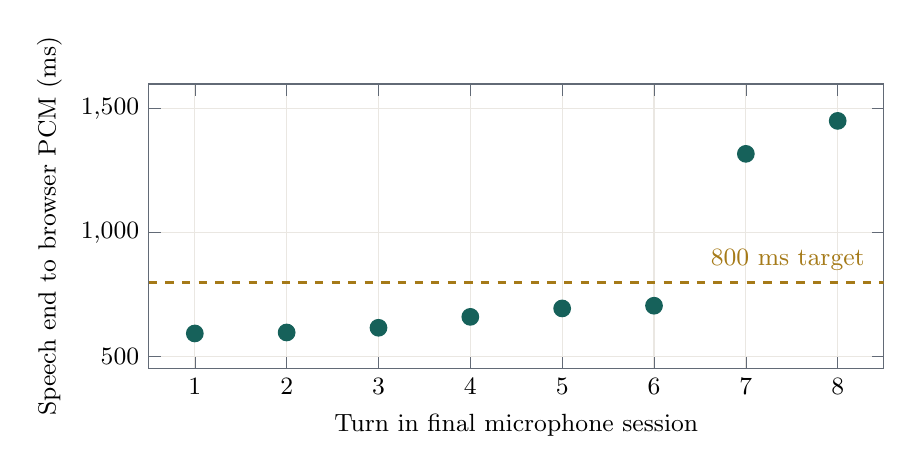
\begin{tikzpicture}
\begin{axis}[
  width=0.9\textwidth,height=5.2cm,
  xlabel={Turn in final microphone session},ylabel={Speech end to browser PCM (ms)},
  xmin=0.5,xmax=8.5,ymin=450,ymax=1600,
  xtick={1,2,3,4,5,6,7,8},
  grid=major,grid style={vlrule!55},axis line style={vlmuted},tick style={vlmuted},
  label style={font=\small},tick label style={font=\small}
]
\addplot[color=vlteal,only marks,mark=*,mark size=3pt] coordinates {
 (1,593) (2,597) (3,616) (4,660) (5,694) (6,705) (7,1318) (8,1451)};
\addplot[color=vlgold,dashed,line width=1.2pt] coordinates {(0.5,800) (8.5,800)};
\node[anchor=south east,font=\small,color=vlgold] at (axis cs:8.4,810) {800 ms target};
\end{axis}
\end{tikzpicture}
\caption{All eight measured turns. Six were below 800 ms; the sample is an acceptance trace, not a
latency distribution.}
\label{fig:human}
\end{figure}

\begin{table}[H]
\centering
\caption{Final human acceptance measurements. Component medians overlap in time and are not
additive.}
\begin{tabularx}{0.72\textwidth}{Xr}
\toprule
Measurement & Observed value \\
\midrule
Completed turns & 8 / 8 \\
Speech end to browser PCM, median & \textbf{677 ms} \\
Speech end to browser PCM, mean & 829 ms \\
Speech end to browser PCM, range & 593--1,451 ms \\
Turns below 800 ms & 6 / 8 \\
Endpoint decision, median & 508 ms \\
LLM first word, median & 268 ms \\
TTS first PCM, median & 453 ms \\
Browser playback, median & 109 ms \\
\bottomrule
\end{tabularx}
\label{tab:latency}
\end{table}

The appropriate conclusion is demonstrated end-to-end operation with promising warm interactive
latency. The sample does not justify a p50 or p95 population claim, nor does it independently
quantify final-topology interruption, duck, or backchannel-resume latency.

\section{Observability and reproducibility}

The browser's diagnostic stream separates model evidence from durable conversation. A rolling
20-second view shows user-speech and assistant-audible lanes together with actual, non-interpolated
completion, floor-take, and non-floor-feedback observations. Each point includes adapter health,
Silero state, applicability, causal audio time, age, and inference latency. Policy events record the
decision, reason, causal source, and decision latency; action events record browser acknowledgment.

\begin{figure}[H]
\centering
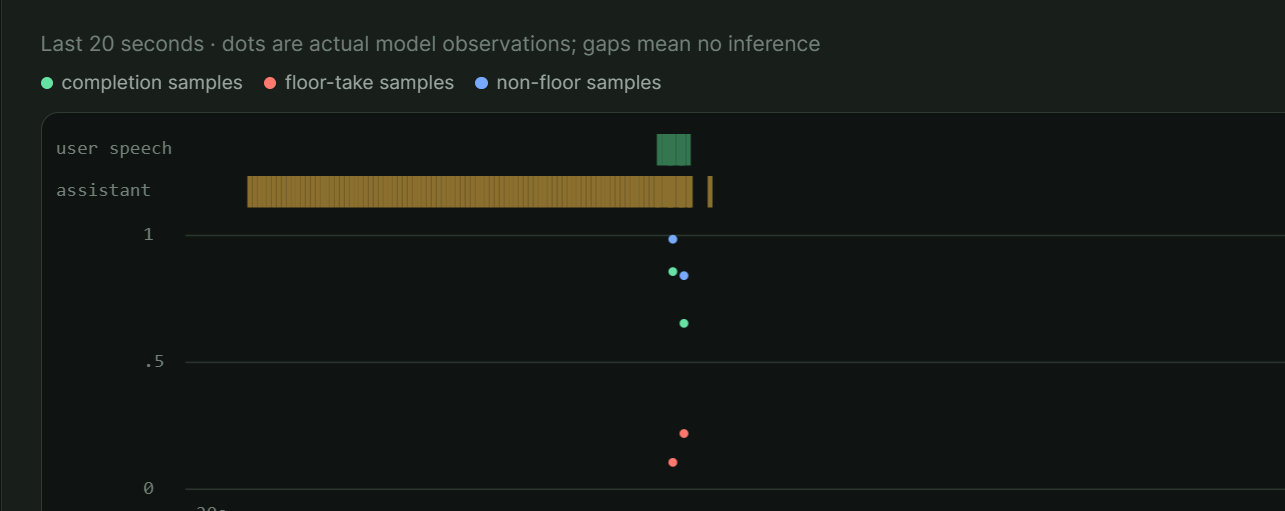
\includegraphics[width=0.95\textwidth]{../assets/voice-agent-interaction-policy.png}
\caption{Public interaction diagnostics. Dots are actual model observations; gaps indicate that no
adapter inference was available at that time.}
\label{fig:debug}
\end{figure}

Reproducibility is expressed at boundaries. Serialized records are frozen, typed, and reject extra
fields. Model names and revisions are pinned. Training manifests retain seeds, input hashes,
configuration, metrics, and checkpoint identity. Evaluation inventories and predictions carry
content hashes and detector provenance; test commands require the validation lock. Deployment
packages the final adapter and mounts persistent model caches without committing credentials.

The public artifacts include the tool-use dataset, LoRA, merged 1.7B checkpoint, and synthetic
turn-taking audio. Human conversational audio remains restricted by its source terms. The source
repository contains the generation, preparation, training, evaluation, runtime, browser, and Modal
deployment code together with detailed runbooks.

\section{Discussion and limitations}

The project produced two useful reversals. First, the smaller language model learned the synthetic
tool protocol but lost too much general quality in live canaries; production uses Qwen3-4B. Second,
the causal adapter learned cross-domain interaction signal but did not provide a competitive sole
endpoint policy; production combines its evidence with immediate Silero timing and conservative
fallbacks. These are not failed integrations. They are examples of evaluation changing a system
before a narrow offline metric became a product claim.

The deployed result still has important limitations:

\begin{itemize}
  \item Cold scale-from-zero readiness is approximately 32--55 seconds despite cached weights and
  concurrent worker loading.
  \item The public service is English-first, admits one session, and depends on a two-GPU Modal
  allocation.
  \item The learned completion head remains conservative; production interaction quality belongs
  to the full hybrid policy, not the adapter alone.
  \item The adapter begins from bounded pre-roll around detected user activity rather than running
  the encoder continuously through assistant-only playback and silence.
  \item Tool selection and factual generation remain fallible. Search depends on an external
  provider secret and tool-result summarization.
  \item Separate bridge and result TTS utterances can retain a small audible seam.
  \item Human evidence is limited to iterative development sessions and one final eight-turn
  acceptance trace, not a blinded multi-participant study.
\end{itemize}

The highest-value next research step is not more synthetic scale. It is a controlled, independently
annotated human evaluation of completion, backchannel, and interruption behavior, with
conversation-level confidence intervals and final-topology action latencies. A new adapter should
only replace the hybrid controller if it improves the latency-versus-false-cancel frontier on that
locked evidence.

\section{Conclusion}

\VoiceLight{} demonstrates a complete path from conversational data work to a public streaming
system. The project generated and published typed synthetic corpora, automatically prepared human
conversation evidence, trained two focused adapters, built locked causal evaluations, restored a
provider-neutral runtime to Modal, and iterated on real microphone behavior until normal turns,
tools, backchannels, interruptions, cancellation, and audible-only history worked together.

Its most defensible outcome is methodological: training metrics were allowed to lose arguments.
The synthetic LoRA remained an artifact when a larger base model sounded better; the turn adapter
became supporting evidence when timing baselines were stronger; GPU placement changed when
component latency exposed contention; and TTS session reuse was reverted when it produced an
audible stall. The resulting hybrid is less ideologically pure and more useful. It also leaves a
clear record of what would need stronger evidence before the next claim or architectural change.

\section*{Artifact links}

\begin{itemize}
  \item Live demo: \url{https://voice.bertil-braun.de}
  \item Source and documentation: \url{https://github.com/BertilBraun/Voice-Light}
  \item Tool-use dataset: \url{https://huggingface.co/datasets/BertilBraun/voice-light-tool-use-synthetic}
  \item Qwen3-1.7B LoRA: \url{https://huggingface.co/BertilBraun/qwen3-1.7b-voice-light-tool-use-lora}
  \item Merged 1.7B checkpoint: \url{https://huggingface.co/BertilBraun/qwen3-1.7b-voice-light-tool-use-merged}
  \item Synthetic turn-taking audio: \url{https://huggingface.co/datasets/BertilBraun/voice-light-synthetic-audio}
\end{itemize}

\begin{thebibliography}{9}
\bibitem{fastconformer}
D. Rekesh et al., ``Fast Conformer with Linearly Scalable Attention for Efficient Speech
Recognition,'' arXiv:2305.05084, 2023. \url{https://arxiv.org/abs/2305.05084}

\bibitem{stateful}
V. Noroozi et al., ``Stateful Conformer with Cache-based Inference for Streaming Automatic Speech
Recognition,'' arXiv:2312.17279, 2023. \url{https://arxiv.org/abs/2312.17279}

\bibitem{vap}
E. Ekstedt and G. Skantze, ``Voice Activity Projection: Self-supervised Learning of Turn-taking
Events,'' arXiv:2205.09812, 2022. \url{https://arxiv.org/abs/2205.09812}

\bibitem{acousticllm}
J. Wang et al., ``Turn-taking and Backchannel Prediction with Acoustic and Large Language Model
Fusion,'' arXiv:2401.14717, 2024. \url{https://arxiv.org/abs/2401.14717}

\bibitem{qwen3}
A. Yang et al., ``Qwen3 Technical Report,'' arXiv:2505.09388, 2025.
\url{https://arxiv.org/abs/2505.09388}

\bibitem{nemotron}
NVIDIA, ``Nemotron Speech Streaming English 0.6B,'' model card, 2026.
\url{https://huggingface.co/nvidia/nemotron-speech-streaming-en-0.6b}

\bibitem{kyutai}
Kyutai, ``Kyutai TTS 1.6B,'' model and implementation documentation, 2025.
\url{https://kyutai.org/tts/}

\bibitem{voice-light}
B. Braun, ``Voice-Light source code, data-generation pipelines, evaluation records, and deployment
documentation,'' 2026. \url{https://github.com/BertilBraun/Voice-Light}
\end{thebibliography}

\end{document}
